\section{Payload Systems and Operation}
\label{sec:Hardware}

\begin{figure}[!ht]
\begin{center}
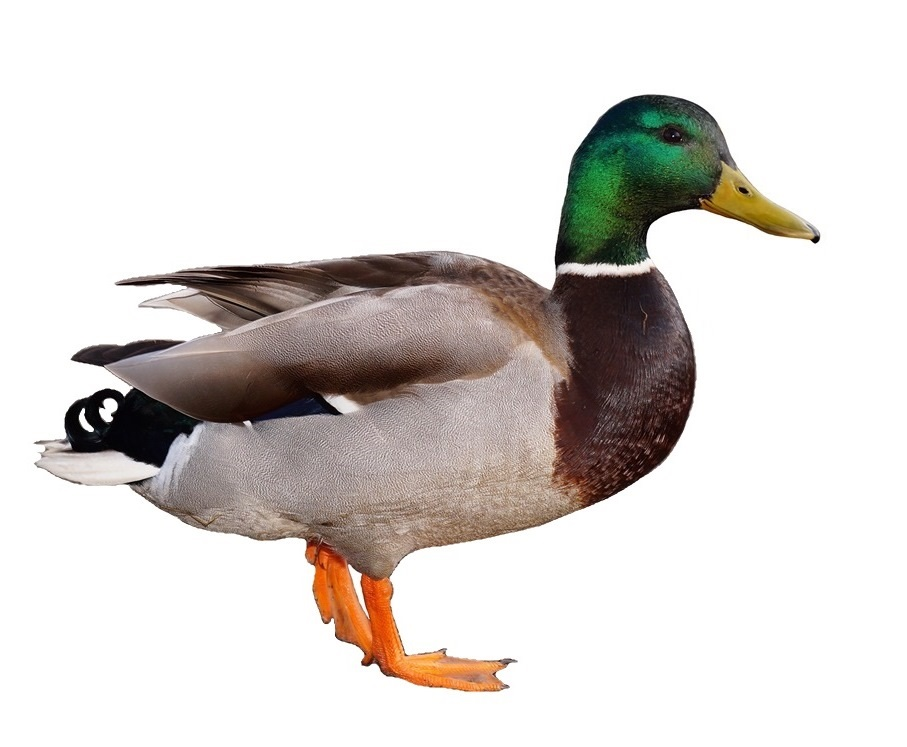
\includegraphics[width=0.8\textwidth]{./Figures/duck.jpg}
\caption{SolidWorks 3D CAD design of the SORA payload.}
\label{fig:payload} 
\end{center}
\end{figure}

SORA 3 will implement an overhauled astrobiology system that will collect larger samples of stratospheric organisms as well as require less amperage, allowing us to expand the radiation system and reduce the chance of electrical failure. The radiation system will apply the techniques developed over the previous missions by consisting of a scintillated MiniPIX within a pressurized module modelled after an ISS module. Additionally, various types of organic photovolatic cells will be flown in order to study their performance in harsh stratospheric conditions.
